\section{講義概要}


\begin{frame}
\frametitle{今日の内容}


微分法の応用に関して解説する. 
\begin{enumerate}
\item 接線と法線の方程式
\item 極値問題, 凹凸, $2$次導関数
\item ロピタルの定理
\end{enumerate} 



\end{frame}




%%%%%%%%%%%%%%%%%%%%%%%%%%%%%%%%%%%%%%%%%%%%%%%%%%%%%%%%%%%%%%%%%%%%%%%%%%%%%%%%%%%%%%%
%%%%%%%%%%%%%%%%%%%%%%%%%%%%%%%%%%%%%%%%%%%%%%%%%%%%%%%%%%%%%%%%%%%%%%%%%%%%%%%%%%%%%%%


%%%%%%%%%%%%%%%%%%%%%%%%%%%%%%%%%%%%%%%%%%%%%%%%%%%%%%%%%%%%%%%%%%%%%%%%%%%%%%%%%%%%%%%
%%%%%%%%%%%%%%%%%%%%%%%%%%%%%%%%%%%%%%%%%%%%%%%%%%%%%%%%%%%%%%%%%%%%%%%%%%%%%%%%%%%%%%%



\section{接線と法線}


\begin{frame}
\frametitle{接線と法線}

\begin{itemize}
\item 関数$f(x)$が$a$で微分可能とは, 点$(a,f(a))$の近傍で$f(x)$のグラフが直線で近似可能であること. 
その直線の傾きは微分係数$f'(a)$で与えられる.  
\item 関数のグラフが直線であれば関数の増加・減少はその傾きの正負で簡単に判定できる.  
そのため, 関数を微分することにより, その関数がどの範囲で増加・減少しているかを解析することが可能になる. 
\end{itemize}

 \begin{figure}[htbp]
 \begin{center} 
  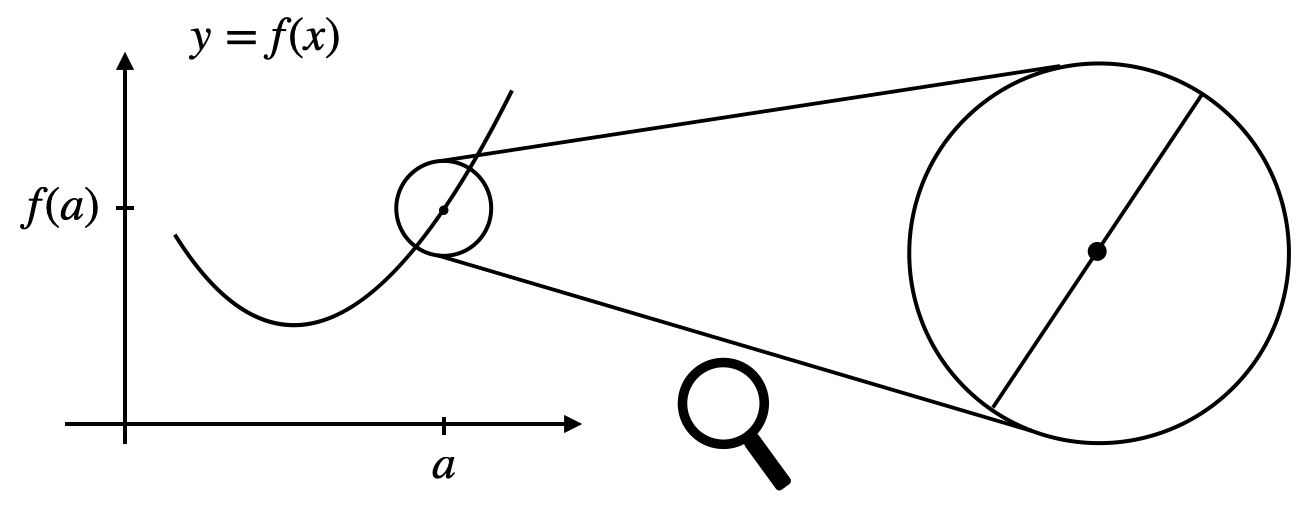
\includegraphics[width=80mm]{calculus7/differentiable2.png}
 \end{center}
\end{figure}




\end{frame}



%%%%%%%%%%%%%%%%%%%%%%%%%%%%%%%%%%%%%%%%%%%%%%%%%%%%%%%%%%%%%%%%%%%%%%%%%%%%%%%%%%%%%%%
%%%%%%%%%%%%%%%%%%%%%%%%%%%%%%%%%%%%%%%%%%%%%%%%%%%%%%%%%%%%%%%%%%%%%%%%%%%%%%%%%%%%%%%





\begin{frame}
\frametitle{接線}

\vspace{-2mm}

\begin{Def}
関数$f(x)$が$a$で微分可能であるとする. 
点$(a,f(a))$を通る傾き$f'(a)$の直線を, $y=f(x)$のグラフの$(a,f(a))$における\underline{接線}という. 
具体的に式で書くと
$$
y-f(a)=f'(a)(x-a). 
$$
\end{Def}
式を整理して
$$
y=f'(a)x + f(a) -f'(a)a
$$
と書くこともできる. 
\vspace{-2mm}

 \begin{figure}[htbp]
 \begin{center} 
  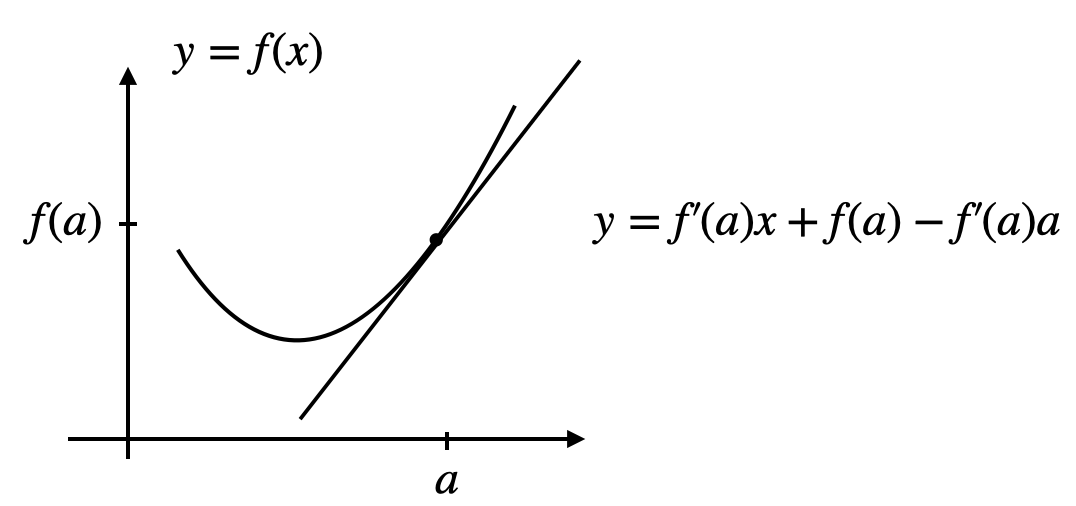
\includegraphics[width=70mm]{calculus7/tangent.png}
 \end{center}
\end{figure}


\end{frame}



%%%%%%%%%%%%%%%%%%%%%%%%%%%%%%%%%%%%%%%%%%%%%%%%%%%%%%%%%%%%%%%%%%%%%%%%%%%%%%%%%%%%%%%
%%%%%%%%%%%%%%%%%%%%%%%%%%%%%%%%%%%%%%%%%%%%%%%%%%%%%%%%%%%%%%%%%%%%%%%%%%%%%%%%%%%%%%%





\begin{frame}
\frametitle{接線}


関数$f(x)=x^2-x-3$のグラフの$(2,f(2))$における接線を求める. \\
\ \\

導関数は$f'(x)=2x-1$である. 
$f(2)=-1$, $f'(2)=3$より, 接線の方程式は
$$
y-(-1)=3(x-2), 
$$
つまり
$$
y=3x-7. 
$$




\end{frame}

%%%%%%%%%%%%%%%%%%%%%%%%%%%%%%%%%%%%%%%%%%%%%%%%%%%%%%%%%%%%%%%%%%%%%%%%%%%%%%%%%%%%%%%
%%%%%%%%%%%%%%%%%%%%%%%%%%%%%%%%%%%%%%%%%%%%%%%%%%%%%%%%%%%%%%%%%%%%%%%%%%%%%%%%%%%%%%%





\begin{frame}
\frametitle{法線}


\begin{Def}
関数$f(x)$が$a$で微分可能であるとする. 
点$(a,f(a))$において, $y=f(x)$のグラフの接線と直交する直線を\underline{法線}という. 
具体的に式で書くと
$$
y-f(a)=-\frac{1}{f'(a)}(x-a). 
$$
\end{Def}
\begin{itemize}
\item 式を整理して
$$
y=-\frac{1}{f'(a)}x + f(a) +\frac{a}{f'(a)}
$$
と書くこともできる.  
\item 傾きが$s$と$t$の直線が直交する条件は$st=-1$である. (非自明)
\end{itemize}

\end{frame}




%%%%%%%%%%%%%%%%%%%%%%%%%%%%%%%%%%%%%%%%%%%%%%%%%%%%%%%%%%%%%%%%%%%%%%%%%%%%%%%%%%%%%%%
%%%%%%%%%%%%%%%%%%%%%%%%%%%%%%%%%%%%%%%%%%%%%%%%%%%%%%%%%%%%%%%%%%%%%%%%%%%%%%%%%%%%%%%





\begin{frame}
\frametitle{法線}


関数$f(x)=x^2-x-3$のグラフの$(2,f(2))$における法線を求める. \\
\ \\

導関数は$f'(x)=2x-1$である. 
$f(2)=-1$, $f'(2)=3$より, 法線の方程式は
$$
y-(-1)=-\frac{1}{3}(x-2), 
$$
つまり
$$
y=-\frac{1}{3}x-\frac{1}{3}.  
$$




\end{frame}




%%%%%%%%%%%%%%%%%%%%%%%%%%%%%%%%%%%%%%%%%%%%%%%%%%%%%%%%%%%%%%%%%%%%%%%%%%%%%%%%%%%%%%%
%%%%%%%%%%%%%%%%%%%%%%%%%%%%%%%%%%%%%%%%%%%%%%%%%%%%%%%%%%%%%%%%%%%%%%%%%%%%%%%%%%%%%%%

\section{極値問題}



\begin{frame}
\frametitle{単調増加, 単調減少}


\begin{Def}
\begin{itemize}
\item 関数$f(x)$は
$$
x_1 < x_2 \ \Rightarrow \ f(x_1)  \le f(x_2)
$$
を満たすとき, \underline{単調増加}と呼ばれ, 
$$
x_1 < x_2 \ \Rightarrow \ f(x_1)  \ge f(x_2)
$$
を満たすとき, \underline{単調減少}と呼ばれる. 
\item $\le$を$<$に置き換えた条件を満たすとき, \underline{狭義単調増加}と呼ばれ, 
$\ge$を$>$に置き換えた条件を満たすとき, \underline{狭義単調減少}と呼ばれる. 
\end{itemize}
\end{Def}




\end{frame}


%%%%%%%%%%%%%%%%%%%%%%%%%%%%%%%%%%%%%%%%%%%%%%%%%%%%%%%%%%%%%%%%%%%%%%%%%%%%%%%%%%%%%%%
%%%%%%%%%%%%%%%%%%%%%%%%%%%%%%%%%%%%%%%%%%%%%%%%%%%%%%%%%%%%%%%%%%%%%%%%%%%%%%%%%%%%%%%



\begin{frame}
\frametitle{単調増加, 単調減少}


関数の増減と微分に関して, 次の関係は基本的である. 

\begin{Thm}
関数$f(x)$が微分可能であるとする. 
\begin{itemize}
\item $f'(x)\ge0$ならば$f(x)$は単調増加. 
\item $f'(x)>0$ならば$f(x)$は狭義単調増加. 
\item $f'(x)\le0$ならば$f(x)$は単調減少. 
\item $f'(x)<0$ならば$f(x)$は狭義単調減少. 
\item $f'(x)=0$ならば$f(x)$は定数. 
\end{itemize}
\end{Thm}
微分係数が接線の傾きを与えていることを思い出せば, 直感的に理解しやすい. 


\end{frame}


%%%%%%%%%%%%%%%%%%%%%%%%%%%%%%%%%%%%%%%%%%%%%%%%%%%%%%%%%%%%%%%%%%%%%%%%%%%%%%%%%%%%%%%
%%%%%%%%%%%%%%%%%%%%%%%%%%%%%%%%%%%%%%%%%%%%%%%%%%%%%%%%%%%%%%%%%%%%%%%%%%%%%%%%%%%%%%%



\begin{frame}
\frametitle{極大・極小}
\vspace{-2.5mm}

\begin{Def}
関数$f(x)$は$a$の近傍($a$を含む小さな開区間)において
\begin{itemize} 
\item $x<a$で単調増加,  $x>a$で単調減少となるとき, $f(x)$は$a$で\underline{極大}であるといい, $f(a)$を\underline{極大値}という.
\item  $x<a$で単調減少,  $x>a$で単調増加となるとき, $f(x)$は$a$で\underline{極小}であるといい, $f(a)$を\underline{極小値}という.
\end{itemize}
\underline{極値}: 極大値と極小値, \underline{極値問題}: 極値を求める問題. 
\end{Def}

関数の最大値と最小値はそれぞれ極大値と極小値. 

\vspace{-1mm}

 \begin{figure}[htbp]
 \begin{center} 
  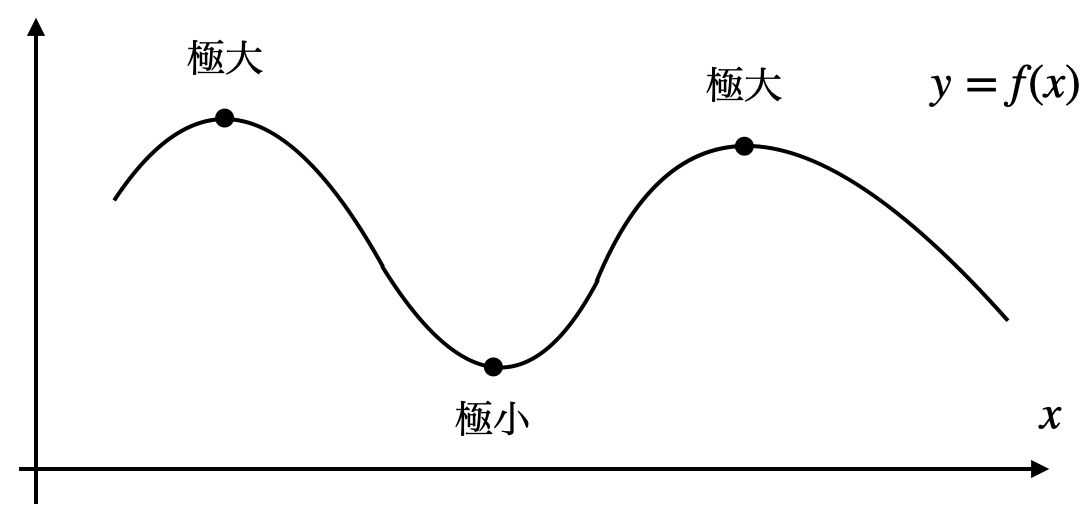
\includegraphics[width=65mm]{calculus7/local_maxmin.png}
 \end{center}
\end{figure}

\end{frame}


%%%%%%%%%%%%%%%%%%%%%%%%%%%%%%%%%%%%%%%%%%%%%%%%%%%%%%%%%%%%%%%%%%%%%%%%%%%%%%%%%%%%%%%
%%%%%%%%%%%%%%%%%%%%%%%%%%%%%%%%%%%%%%%%%%%%%%%%%%%%%%%%%%%%%%%%%%%%%%%%%%%%%%%%%%%%%%%



\begin{frame}
\frametitle{ワイエルシュトラスの定理}



連続関数の最大値と最小値に関しては次の定理が知られている. 

\begin{Thm}[ワイエルシュトラスの定理] \label{Weierstrass}
関数$f(x)$が$[a,b]$で連続であるとき, $c,d\in [a,b]$が存在して, 任意の$x \in [a,b]$に対して
$$
f(x) \le f(c), \ \ \ f(d) \le f(x). 
$$
つまり, $f(x)$は$[a,b]$において$c$で最大値$f(c)$, $d$で最小値$f(d)$をとる. 
\end{Thm}
\begin{itemize}
\item 定理\ref{Weierstrass}は関数が具体的にどこで最大値と最小値をとるのかについてまでは教えてくれない. 
\item 連続性を仮定するのは何故であろうか? 
\end{itemize}
\end{frame}

%%%%%%%%%%%%%%%%%%%%%%%%%%%%%%%%%%%%%%%%%%%%%%%%%%%%%%%%%%%%%%%%%%%%%%%%%%%%%%%%%%%%%%%
%%%%%%%%%%%%%%%%%%%%%%%%%%%%%%%%%%%%%%%%%%%%%%%%%%%%%%%%%%%%%%%%%%%%%%%%%%%%%%%%%%%%%%%



\begin{frame}
\frametitle{極大・極小}


\begin{Def}
関数$f(x)$が微分可能であるとき, $f'(a)=0$なる$a$を$f(x)$の\underline{停留点}という. 
\end{Def}

\begin{itemize}
\item $f(x)$が$a$で極大・極小であれば$a$は$f(x)$の停留点である. 
\begin{itemize}
\item 極大: $f'(x)$の符号が$a$で正から負に変化
\item 極小: $f'(x)$の符号が$a$で負から正に変化
\end{itemize}
\item 停留点は極大・極小とは限らない. 実際, $f(x)=x^3$の停留点$a=0$は極大でも極小でもない. 
\item 極値問題では, 導関数を計算して停留点を求め, それが極大・極小を与えているか確認する, という方法を採る. 
\end{itemize}
\end{frame}



%%%%%%%%%%%%%%%%%%%%%%%%%%%%%%%%%%%%%%%%%%%%%%%%%%%%%%%%%%%%%%%%%%%%%%%%%%%%%%%%%%%%%%%
%%%%%%%%%%%%%%%%%%%%%%%%%%%%%%%%%%%%%%%%%%%%%%%%%%%%%%%%%%%%%%%%%%%%%%%%%%%%%%%%%%%%%%%



\begin{frame}
\frametitle{増減表}

増減表: 関数の増減と極値に関して纏めた表.\\
\ \\

$f(x)=2x^2+8x+13$に関して, 
$$
f'(x)=4x+8=4(x+2) \vspace{-4.5mm}
$$
\begin{itemize}
\item $f'(x)<0 \ \Leftrightarrow \ x<-2$, 
\item $f'(x)=0 \ \Leftrightarrow \ x=-2$, 
\item $f'(x)>0 \ \Leftrightarrow \ x>-2$, 
\end{itemize}

\begin{table}[htb]
\begin{center}
\begin{tabular}{c|c|c|c}
$x$ & $\dots$ & $-2$ & $\dots$ \\ \hline 
$f'(x)$   & $-$ & 0  & $+$   \\ \hline 
$f(x)$   & $\searrow$ & $5$ &  $\nearrow$  
  \end{tabular}
  \end{center}
\end{table}

\end{frame}




%%%%%%%%%%%%%%%%%%%%%%%%%%%%%%%%%%%%%%%%%%%%%%%%%%%%%%%%%%%%%%%%%%%%%%%%%%%%%%%%%%%%%%%
%%%%%%%%%%%%%%%%%%%%%%%%%%%%%%%%%%%%%%%%%%%%%%%%%%%%%%%%%%%%%%%%%%%%%%%%%%%%%%%%%%%%%%%



\begin{frame}
\frametitle{増減表}

$f(x)=x^3+3x^2-9x+6$に関して, 
$$
f'(x)=3x^2+6x-9=3(x+3)(x-1) \vspace{-4.5mm}
$$
\begin{itemize}
\item $f'(x)<0 \ \Leftrightarrow \ -3<x<1$, 
\item $f'(x)=0 \ \Leftrightarrow \ x=-3,1$, 
\item $f'(x)>0 \ \Leftrightarrow \ x<-3 \ \text{or} \ x>1$, 
\end{itemize}

\begin{table}[htb]
\begin{center}
\begin{tabular}{c|c|c|c|c|c}
$x$ & $\dots$ & $-3$ & $\dots$ & 1 & \dots \\ \hline 
$f'(x)$   & $+$ & $0$  & $-$  & $0$ & $+$   \\ \hline 
$f(x)$   & $\nearrow$  & $33$ & $\searrow$  & $1$ &  $\nearrow$  
  \end{tabular}
  \end{center}
\end{table}

\end{frame}


%%%%%%%%%%%%%%%%%%%%%%%%%%%%%%%%%%%%%%%%%%%%%%%%%%%%%%%%%%%%%%%%%%%%%%%%%%%%%%%%%%%%%%%
%%%%%%%%%%%%%%%%%%%%%%%%%%%%%%%%%%%%%%%%%%%%%%%%%%%%%%%%%%%%%%%%%%%%%%%%%%%%%%%%%%%%%%%



\begin{frame}
\frametitle{関数の凹凸}


\begin{Def}
開区間$I$において, 関数$f(x)$が
\begin{itemize}
\item \underline{下に凸}: 任意の$x_1,x_2 \in I$と$0 \le \lambda \le 1$に対して
$$
\lambda f(x_1)+(1-\lambda)f(x_2) \ge f(\lambda x_1+(1-\lambda)x_2). 
$$
\item \underline{上に凸}: 任意の$x_1,x_2 \in I$と$0 \le \lambda \le 1$に対して
$$
\lambda f(x_1)+(1-\lambda)f(x_2) \le f(\lambda x_1+(1-\lambda)x_2). 
$$
\end{itemize}
\end{Def}

点$p,q$に対して, $\lambda p+(1-\lambda)q$は点$p,q$間を$\lambda:(1-\lambda)$に内分する点. 


\end{frame}


%%%%%%%%%%%%%%%%%%%%%%%%%%%%%%%%%%%%%%%%%%%%%%%%%%%%%%%%%%%%%%%%%%%%%%%%%%%%%%%%%%%%%%%
%%%%%%%%%%%%%%%%%%%%%%%%%%%%%%%%%%%%%%%%%%%%%%%%%%%%%%%%%%%%%%%%%%%%%%%%%%%%%%%%%%%%%%%



\begin{frame}
\frametitle{関数の凹凸}


関数の凹凸は視覚的に理解するのが良い. 
グラフ上の2点を結んだ線分が常にグラフの上側(下側)にあるような関数が下に凸(上に凸).


 \begin{figure}[htbp]
 \begin{center} 
  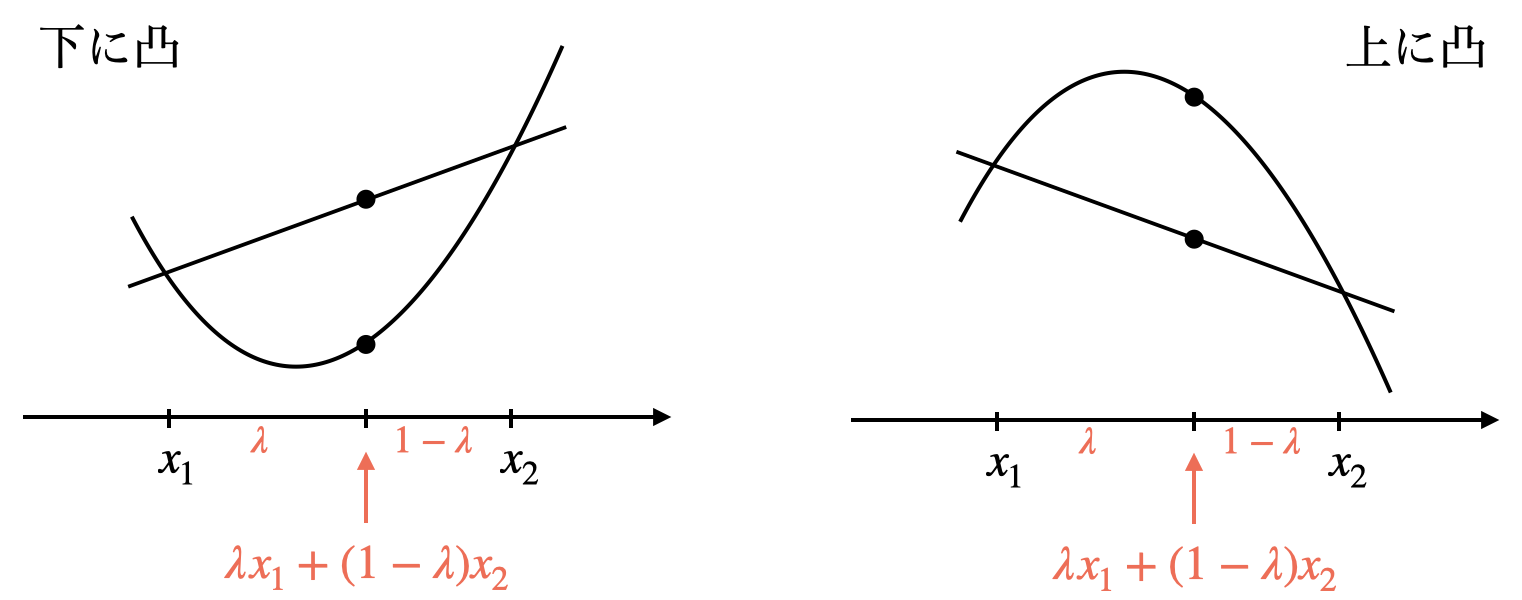
\includegraphics[width=100mm]{calculus7/convex.png}
 \end{center}
\end{figure}


\end{frame}



%%%%%%%%%%%%%%%%%%%%%%%%%%%%%%%%%%%%%%%%%%%%%%%%%%%%%%%%%%%%%%%%%%%%%%%%%%%%%%%%%%%%%%%
%%%%%%%%%%%%%%%%%%%%%%%%%%%%%%%%%%%%%%%%%%%%%%%%%%%%%%%%%%%%%%%%%%%%%%%%%%%%%%%%%%%%%%%



\begin{frame}
\frametitle{関数の凹凸}


その点の左右で上に凸と下に凸とが切り替わるような点を\underline{変曲点}という.


 \begin{figure}[htbp]
 \begin{center} 
  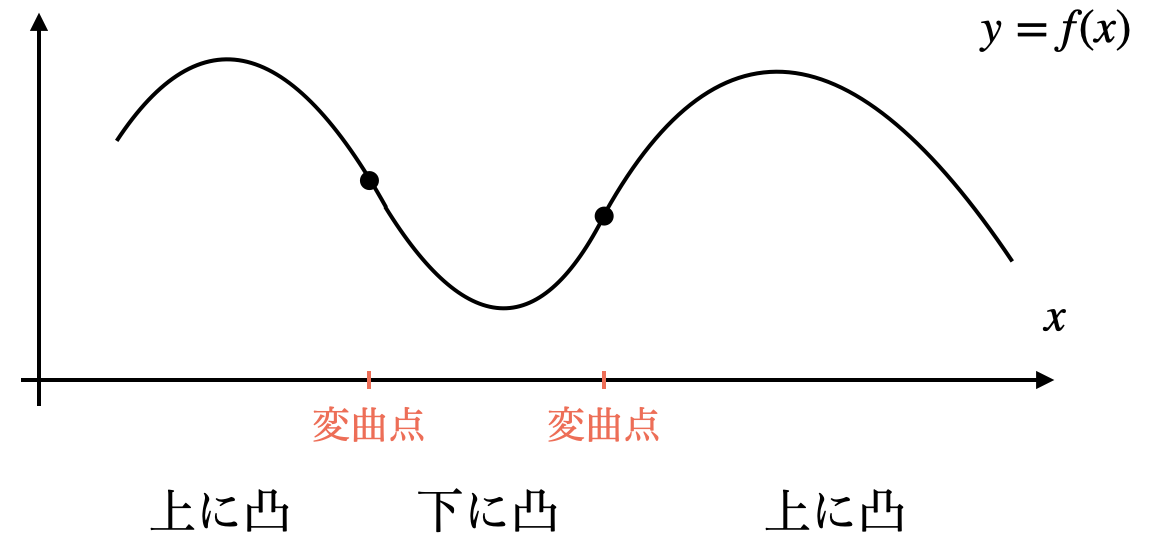
\includegraphics[width=85mm]{calculus7/inflection.png}
 \end{center}
\end{figure}


\end{frame}


%%%%%%%%%%%%%%%%%%%%%%%%%%%%%%%%%%%%%%%%%%%%%%%%%%%%%%%%%%%%%%%%%%%%%%%%%%%%%%%%%%%%%%%
%%%%%%%%%%%%%%%%%%%%%%%%%%%%%%%%%%%%%%%%%%%%%%%%%%%%%%%%%%%%%%%%%%%%%%%%%%%%%%%%%%%%%%%



\begin{frame}
\frametitle{2次導関数}


関数の増減は微分することで判定ができた. 
次に関数の凹凸は$2$回微分することにより判定できることを説明する. 

\begin{Def}
関数$f(x)$の導関数$f'(x)$も微分可能であるとき, $f(x)$は\underline{$2$回微分可能}であるという. 
$f'(x)$の導関数を$f''(x)$と書き, $f(x)$の\underline{$2$次導関数}と呼ぶ. 
\end{Def}

$f(x)$が位置を表すとき, 
\begin{itemize}
\item $f'(x)$は速度(=位置の変化率), 
\item $f''(x)$は加速度(=速度の変化率) 
\end{itemize}
を表す.
\end{frame}


%%%%%%%%%%%%%%%%%%%%%%%%%%%%%%%%%%%%%%%%%%%%%%%%%%%%%%%%%%%%%%%%%%%%%%%%%%%%%%%%%%%%%%%
%%%%%%%%%%%%%%%%%%%%%%%%%%%%%%%%%%%%%%%%%%%%%%%%%%%%%%%%%%%%%%%%%%%%%%%%%%%%%%%%%%%%%%%



\begin{frame}
\frametitle{2次導関数}
\vspace{-2mm}

\begin{Thm}
$f(x)$は$2$回微分可能とする. 
\begin{itemize}
\item $f''(x)>0$ならば$f(x)$は下に凸. 
\item $f''(x)<0$ならば$f(x)$は上に凸.
\item 変曲点$a$は$2$階微分の符号が変化する点. 特に$f''(a)=0$
\end{itemize}
\end{Thm}
$f''(x)>0$は接線の傾きが増加すること, $f''(x)<0$は接線の傾きが減少することを意味する. 

\vspace{-1mm}

 \begin{figure}[htbp]
 \begin{center} 
  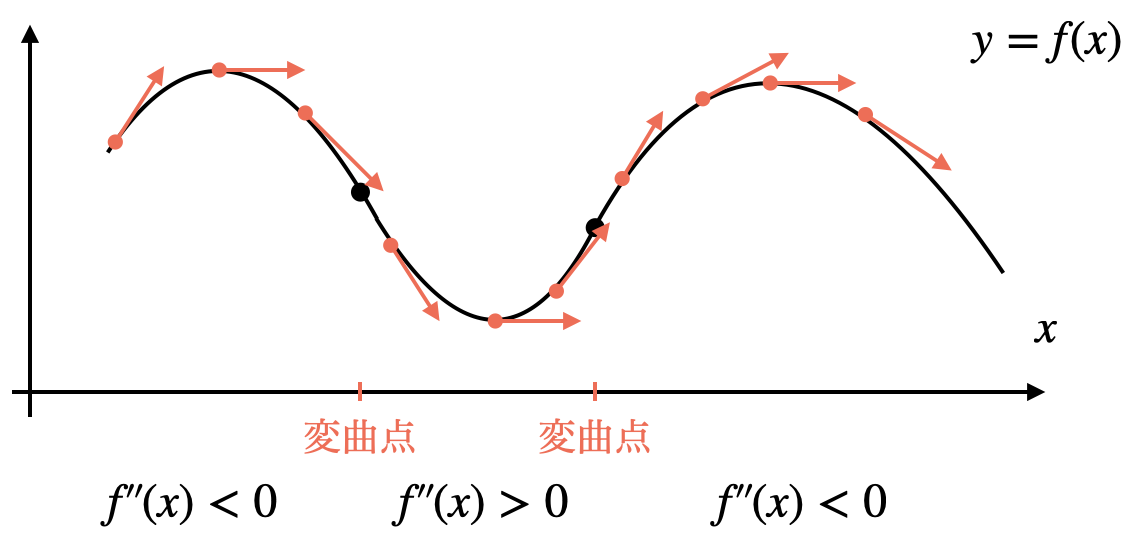
\includegraphics[width=85mm]{calculus7/inflection2.png}
 \end{center}
\end{figure}

\end{frame}


%%%%%%%%%%%%%%%%%%%%%%%%%%%%%%%%%%%%%%%%%%%%%%%%%%%%%%%%%%%%%%%%%%%%%%%%%%%%%%%%%%%%%%%
%%%%%%%%%%%%%%%%%%%%%%%%%%%%%%%%%%%%%%%%%%%%%%%%%%%%%%%%%%%%%%%%%%%%%%%%%%%%%%%%%%%%%%%



\begin{frame}
\frametitle{正規分布の変曲点}
%https://manabitimes.jp/math/1214

正数$a>0$に関して, $f(x)=e^{-ax^2}$の変曲点を求める. 
\begin{align*}
f'(x) & = -2axe^{-ax^2} \\
f''(x) & = -2ae^{-ax^2} + (-2ax)^2e^{-ax^2} \\
&= 2ae^{-ax^2} (2ax^2-1)
\end{align*}
これより$x=\pm \frac{1}{\sqrt{2a}}$が変曲点. \\
\ \\

特に$a=\frac{1}{2\sigma^2}$とすると, $x=\pm \sigma$が変曲点. 

\end{frame}




%%%%%%%%%%%%%%%%%%%%%%%%%%%%%%%%%%%%%%%%%%%%%%%%%%%%%%%%%%%%%%%%%%%%%%%%%%%%%%%%%%%%%%%
%%%%%%%%%%%%%%%%%%%%%%%%%%%%%%%%%%%%%%%%%%%%%%%%%%%%%%%%%%%%%%%%%%%%%%%%%%%%%%%%%%%%%%%



\begin{frame}
\frametitle{正規分布の変曲点 (発展)}

\begin{Thm}
正規分布の確率密度関数$f(x)=\frac{1}{\sqrt{2 \pi \sigma}}e^{-\frac{(x-\mu)^2}{2\sigma^2}}$の変曲点は$x=\mu \pm \sigma$. 
\end{Thm}
$\sigma$は正規分布の標準偏差と呼ばれる. 


 \begin{figure}[htbp]
 \begin{center} 
  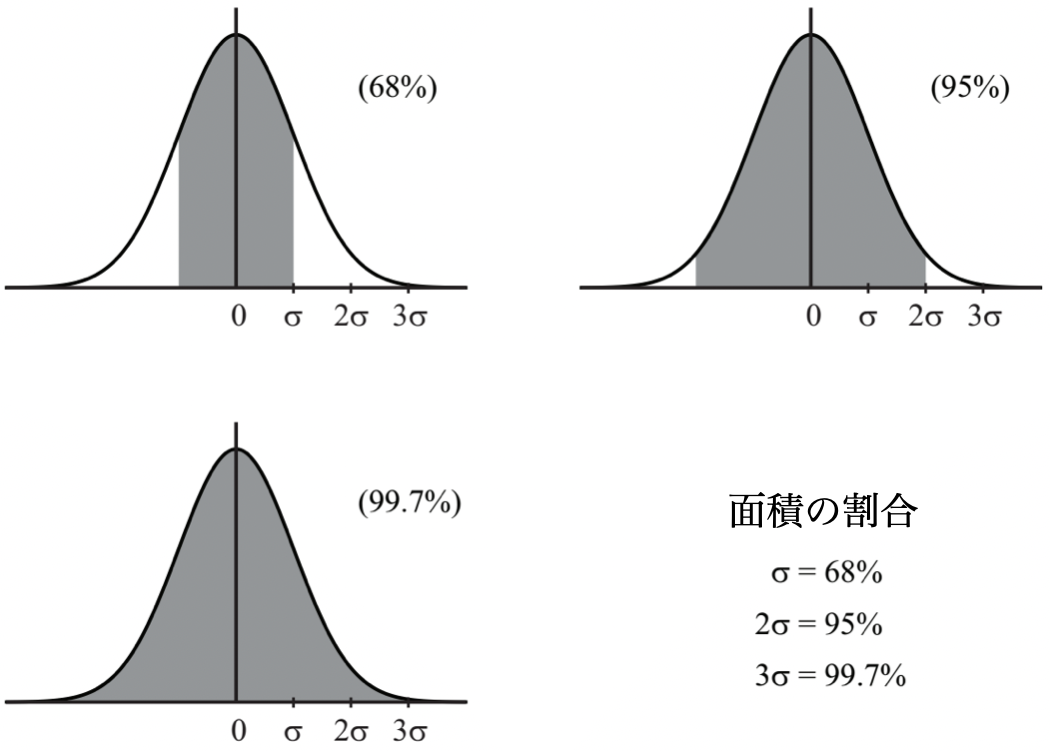
\includegraphics[width=65mm]{calculus7/normal_sigma.png}
 \end{center}
\end{figure}

\end{frame}

%%%%%%%%%%%%%%%%%%%%%%%%%%%%%%%%%%%%%%%%%%%%%%%%%%%%%%%%%%%%%%%%%%%%%%%%%%%%%%%%%%%%%%%
%%%%%%%%%%%%%%%%%%%%%%%%%%%%%%%%%%%%%%%%%%%%%%%%%%%%%%%%%%%%%%%%%%%%%%%%%%%%%%%%%%%%%%%



\begin{frame}
\frametitle{2次導関数}

停留点は極値とは限らなかったが, $2$次導関数を使うことで, 極大・極小についての判定が可能となる. 


\begin{Thm} \label{2回微分と極値}
$f(x)$は$2$回微分可能とする. 
\begin{itemize}
\item $f'(a)=0$かつ$f''(a)>0$ならば$f(x)$は$a$において極小. 
\item $f'(a)=0$かつ$f''(a)<0$ならば$f(x)$は$a$において極大.  
\end{itemize}
\end{Thm}

\begin{itemize}
\item $f'(a)=f''(a)=0$である場合には, 定理\ref{2回微分と極値}からは何も分からない. 
\item 実際, $f(x)=x^3$に関して, $f'(0)=f''(0)=0$であり, $f(x)$は原点$0$において極値をとらない.  
\end{itemize}
\end{frame}


%%%%%%%%%%%%%%%%%%%%%%%%%%%%%%%%%%%%%%%%%%%%%%%%%%%%%%%%%%%%%%%%%%%%%%%%%%%%%%%%%%%%%%%
%%%%%%%%%%%%%%%%%%%%%%%%%%%%%%%%%%%%%%%%%%%%%%%%%%%%%%%%%%%%%%%%%%%%%%%%%%%%%%%%%%%%%%%



\begin{frame}
\frametitle{増減凹凸表}

増減凹凸表: 関数の増減, 凹凸, 極値に関して纏めた表.\\
\ \\

$f(x)=x^3+3x^2-9x+6$に関して, 
\begin{align*}
f'(x) &= 3x^2+6x-9=3(x+3)(x-1) \\
f''(x) &= 6x+6=6(x+1)\vspace{-4.5mm}
\end{align*}

これより$f(x)$の増減凹凸表は次で与えられる. 

\begin{table}[htb]
\begin{center}
\begin{tabular}{c|c|c|c|c|c|c|c}
$x$ & $\dots$ & $-3$ & $\dots$ & $-1$ & \dots & 1 & \dots \\ \hline 
$f'(x)$   & $+$ & $0$  & $-$ & $-$ & $-$  & $0$ & $+$   \\ \hline 
$f ''(x)$   & $-$ & $-$  & $-$ & $0$ &  $+$ & $+$  & $+$   \\ \hline 
$f(x)$   & \nel  & $33$ & \sel & $17$ & \ser &  $1$  & \ner   
  \end{tabular}
  \end{center}
\end{table}

\end{frame}



%%%%%%%%%%%%%%%%%%%%%%%%%%%%%%%%%%%%%%%%%%%%%%%%%%%%%%%%%%%%%%%%%%%%%%%%%%%%%%%%%%%%%%%
%%%%%%%%%%%%%%%%%%%%%%%%%%%%%%%%%%%%%%%%%%%%%%%%%%%%%%%%%%%%%%%%%%%%%%%%%%%%%%%%%%%%%%%



\begin{frame}
\frametitle{増減凹凸表}

\begin{Prob}
$x>0$に対して定義される関数$f(x)=x\log x$の増減凹凸表を作り, $f(x)$のグラフを描け. 
\end{Prob}

\vspace{5.5cm}

\end{frame}

%%%%%%%%%%%%%%%%%%%%%%%%%%%%%%%%%%%%%%%%%%%%%%%%%%%%%%%%%%%%%%%%%%%%%%%%%%%%%%%%%%%%%%%
%%%%%%%%%%%%%%%%%%%%%%%%%%%%%%%%%%%%%%%%%%%%%%%%%%%%%%%%%%%%%%%%%%%%%%%%%%%%%%%%%%%%%%%


\begin{frame}
\frametitle{最適化問題}   

\begin{itemize}
\item 等周問題: 周の長さが$l$の長方形の中で面積を最大にするものは? 
\item 面積$A(x)=x(l/2-x)$
$$
A'(x)=\frac{l}{2}-2x, \ \ \ A''(x)=-2. 
$$
\end{itemize}

 \begin{figure}[htbp]
 \begin{center} 
  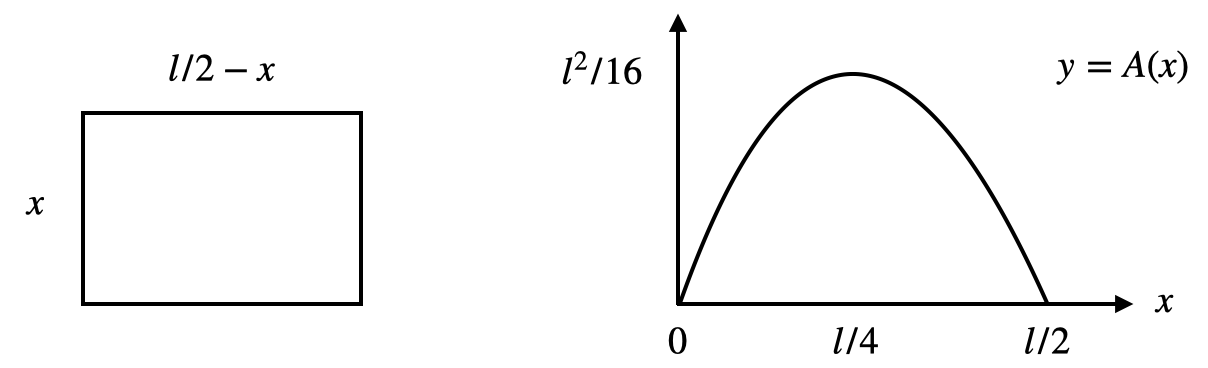
\includegraphics[width=90mm]{calculus7/LecArea.png}
 \end{center}
\end{figure}

\end{frame}




%%%%%%%%%%%%%%%%%%%%%%%%%%%%%%%%%%%%%%%%%%%%%%%%%%%%%%%%%%%%%%%%%%%%%%%%%%%%%%%%%%%%%%%
%%%%%%%%%%%%%%%%%%%%%%%%%%%%%%%%%%%%%%%%%%%%%%%%%%%%%%%%%%%%%%%%%%%%%%%%%%%%%%%%%%%%%%%

%%%%%%%%%%%%%%%%%%%%%%%%%%%%%%%%%%%%%%%%%%%%%%%%%%%%%%%%%%%%%%%%%%%%%%%%%%%%%%%%%%%%%%%
%%%%%%%%%%%%%%%%%%%%%%%%%%%%%%%%%%%%%%%%%%%%%%%%%%%%%%%%%%%%%%%%%%%%%%%%%%%%%%%%%%%%%%%





%%%%%%%%%%%%%%%%%%%%%%%%%%%%%%%%%%%%%%%%%%%%%%%%%%%%%%%%%%%%%%%%%%%%%%%%%%%%%%%%%%%%%%%
%%%%%%%%%%%%%%%%%%%%%%%%%%%%%%%%%%%%%%%%%%%%%%%%%%%%%%%%%%%%%%%%%%%%%%%%%%%%%%%%%%%%%%%




\section{今日のまとめ}
\begin{frame}
\frametitle{まとめ}   


\begin{enumerate}
\item 接線と法線の方程式、
\item 極値問題, 凹凸, 2次導関数
\end{enumerate} 

\end{frame}
